\chapter{Badania wstępne}
\label{cha:Badania wstępne}

Analiza rozpatrywanego problemu detekcji wraz ze sprzętową implementacją pozwala na zaproponowanie możliwych rozwiązań. W niniejszym rozdziale zostaną przedstawione propozycje architektur sieci, proces ich uczenia a także kwantyzacji. 

\section{Architektura wstępna} %section{Architektura wstępna}

%}
% Liczba parametrów sieci \emph{Ultra\_net} wynosi ponad 200 tys..
Liczba parametrów sieci \emph{SkyNet}\footnote{W wersji bez połączenia typu \emph{bypass}} wynosi ponad $300$ tys. 
Zastosowanie separowalnych konwolucji skutkuje znaczną redukcją liczby parametrów względem architektury wykorzystującej pełną konwolucję - powyżej $2.6$ miliona parametrów \footnote{Architektur tych nie można w pełni ze sobą utożsamiać jako substytutów.}. 
Tak znaczna redukcja (również złożoności obliczeniowej) skłania do zastosowania konwolucji separowalnych dla sprzętowej akceleracji. 
W tym celu rozważono architekturę sieci o 9 warstwach konwolucji separowalnej (z bias) z funkcją aktywacji $ReLU$ po konwolucji typu pointwise. Architektura posiada również warstwy Max Pooling po każdej konwolucji separowalnej.
Ostatnia warstwa stanowi warstwę podobną do warstwy \emph{YOLOv1}. Na rysunku \ref{fig:arch_v1} przedstawiono graficzną reprezentację architektury. 
Jako wejście sieci pozostawiono oryginalne wymiary obrazów dostępnych w zbiorze treningowym.

Ze względu, iż rozpatrywany problem to detekcja bez klasyfikacji, pominięto w funkcji błędu \eqref{eq:lossv1} część związaną z klasyfikacją. 
Jako wartości referencyjne dla wyjść sieci wykorzystano maskę $y_{ref}$ (o wymiarach 5x7x12) z odpowiadającymi wartościami dla kanałów. Równania \eqref{eq:y_ref_valv1}-\eqref{eq:y_ref_hv1} prezentują sposób wyznaczenia wartości referencyjnych dla elementów poszczególnych kanałów. 

\begin{figure}
    \centering
    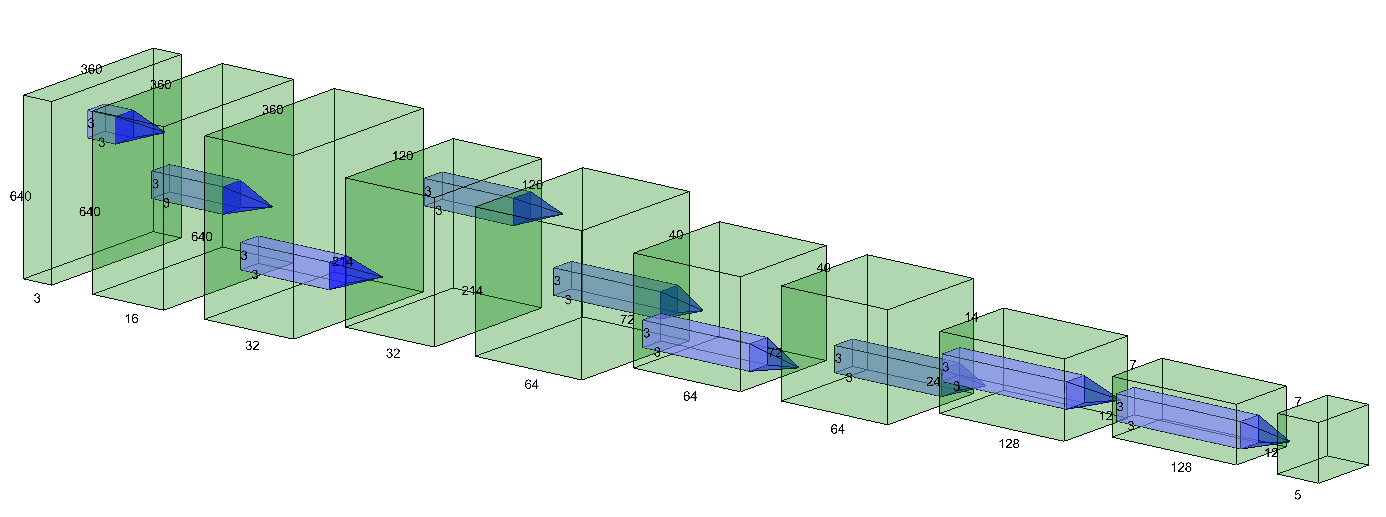
\includegraphics[width=\linewidth]{images/arch_v1.png}
    \caption{Wstępna architektura sieci dla zadania detekcji, wykorzystująca konwolucje separowalne oraz warstwę podobną do \emph{YOLOv1}. Architektura posiada niespełna 43 tys. parametrów.}
    \label{fig:arch_v1}
\end{figure}

\begin{equation}
y_{ref}_{0,i,j} = 
\begin{cases}
    1, & \text{if }  i = row \And j = col \\
    0,              & \text{otherwise}
\end{cases}
\label{eq:y_ref_valv1}
\end{equation}

\begin{equation}
y_{ref}_{1,i,j} = 
\begin{cases}
    x_c \frac{12}{640} - col - 0.5, & \text{if }  i = row \And j = col \\
    0,              & \text{otherwise}
\end{cases}
\label{eq:y_ref_xv1}
\end{equation}

\begin{equation}
y_{ref}_{2,i,j} = 
\begin{cases}
    y_c \frac{7}{360} - row - 0.5, & \text{if }  i = row \And j = col \\
    0,              & \text{otherwise}
\end{cases}
\label{eq:y_ref_yv1}
\end{equation}

\begin{equation}
y_{ref}_{3,i,j} = 
\begin{cases}
    log(\frac{w}{a_w}) & \text{if }  i = row \And j = col \\
    0,              & \text{otherwise}
\end{cases}
\label{eq:y_ref_wv1}
\end{equation}

\begin{equation}
y_{ref}_{4,i,j} = 
\begin{cases}
    log(\frac{h}{a_h}) & \text{if }  i = row \And j = col \\
    0,              & \text{otherwise}
\end{cases}
\label{eq:y_ref_hv1}
\end{equation}

$row$ oraz $col$ oznaczają indeks siatki wyjściowej do którego został przypisany referencyjny obiekt, $a_w$ oraz $a_h$ odpowiednio szerokość i wysokość \emph{anchor box}. 
Przyjęto  $a_w = 16$ oraz $a_h = 16$ jako wartość łączna wartość kroku sieci (ang. \emph{stride}) wynikająca z liczby warstw Max Pooling.
Przyjmując za $x_c, y_c, w, h$ odpowiednio współrzędne położenia środka obiektu oraz jego wymiary, można wyznaczyć indeksy $row$ oraz $col$ według wzorów \eqref{eq:rowv1}-\eqref{eq:colv1}.

\begin{equation}
col = \round{x_c \frac{12}{640} - 0.5}
\label{eq:colv1}
\end{equation}
\begin{equation}
row = \round{y_c \frac{7}{360} - 0.5}
\label{eq:rowv1}
\end{equation}


Błąd wykrycia obiektu został zdefiniowany jako entropia binarna $BCE$. 
Błąd przesunięcia od centrum siatki detekcji (wynikającej z wymiarów ostatniej warstwy) został zdefiniowany jako średni błąd bezwzględny $MAE$. Błąd wymiarów został zdefiniowany jako wartość średnia pierwiastka $MSQRT$ z wartości bezwzględnej różnicy pomiędzy odpowiedzią sieci oraz wartością referencyjną.
Funkcję błędu (reprezentowaną przez równanie \eqref{eq:lossv1}) dla całej sieci stanowi ważona suma błędów składowych ze współczynnikami $\lambda_obj, \lambda_xy oraz \lambda_wh$. 

\begin{equation}
\begin{aligned}
loss =& \lambda_{obj} BCE(\sigma(y_{pred}_{0,:,:}), y_{ref}_{0,:,:}) \\
&+ \frac{\lambda_{xy}}{2}( MAE(y_{pred}_{1,:,:}, y_{ref}_{1,:,:}) + MAE(y_{pred}_{2,:,:}, y_{ref}_{2,:,:})) \\
&+ \frac{\lambda_{wh}}{2} (MSQRT(|y_{pred}_{3,:,:} - y_{ref}_{3,:,:}|) + MSQRT(|y_{pred}_{4,:,:} - y_{ref}_{4,:,:}|))
\end{aligned}
\label{eq:lossv1}
\end{equation}


Przed rozpoczęciem procesu uczenia dokonano podziału dostępnego zbioru uczącego na trzy zbiory: uczący, walidacyjny oraz testowy w stosunku 81:9:10. Podział został przeprowadzony losowo wewnątrz każdej sekwencji.
Uzyskany podział zbioru był stosowany dla wszystkich dalszych wariantów architektur i funkcji błędu.

Rozpoczynając trening sieci ustalono wszystkie parametry funkcji błędu \eqref{eq:lossv1} na wartość $1$.
Dla zbioru uczącego przeprowadzano augmentację danych\footnote{Dla pozostałych wariantów architektur również przeprowadzano augmentację danych.} z wykorzystaniem filtracji uśredniającej, zakłóceń addytywnych, przeskalowania czy też rotacji.
Do minimalizacji błędu użyto algorytmu \emph{Adadelta}\footnote{Dla pozostałych architektur również użyto tego algorytmu.}.

Proces uczenia przerwano, gdy nie zauważono zmian wartości błędu oraz metryki IoU dla zbioru uczącego oraz walidacyjnego.
Finalnie architektura osiągnęła wartość współczynnika $iou = 0.47$ dla zbioru walidacyjnnego.

\section{Architektura rozgałęziona}
Ze względu na niewielką wartość współczynnika $iou$, architekturę zmodyfikowano o dodanie dodatkowego wyjścia z sieci pochodzącego z warstwy pośredniej zakończonego warstwą analogicznie do wersji nierozgałęzionej (wymiary \emph{anchor box} dla rozgałęzienia $a_w = 8$ oraz  $a_h = 8$). Na rysunku \ref{fig:arch_v2} przedstawiono graficzną reprezentację architektury. Po przeprowadzeniu procesu ucznia sieci, z wykorzystaniem techniki transferu wiedzy z architektury pierwotnej, uzyskano pogorszenie wartości $iou$. 

\begin{figure}
    \centering
    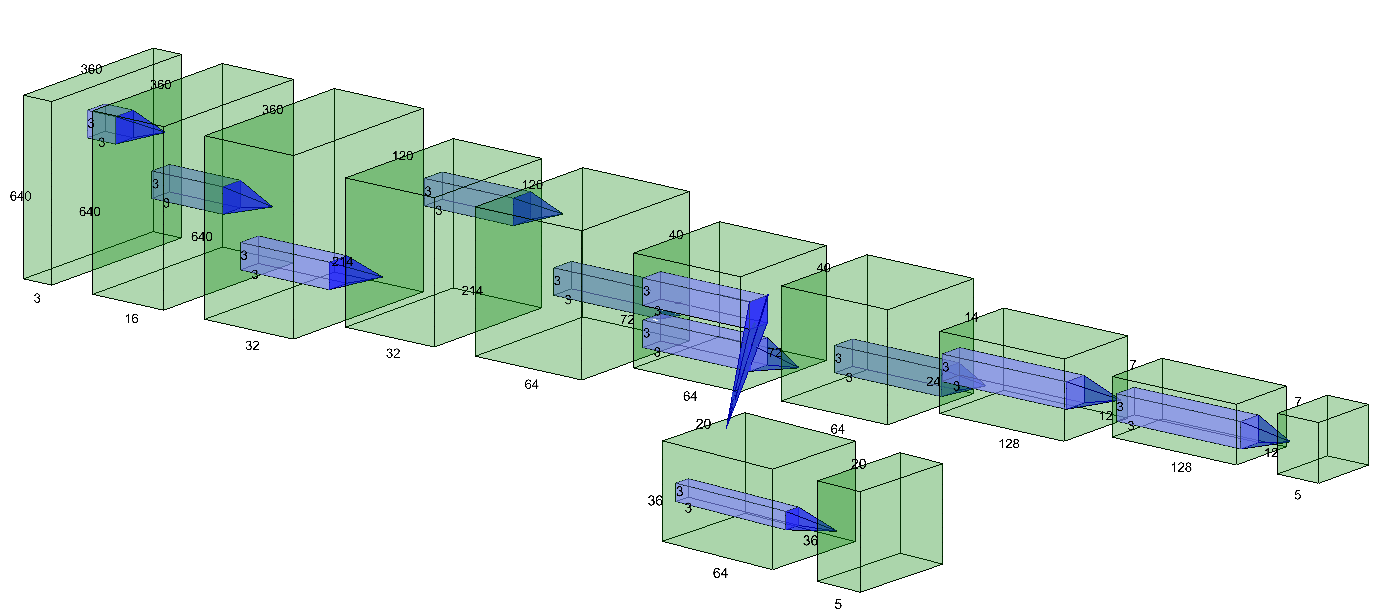
\includegraphics[width=\linewidth]{images/Architektura_branched.png}
    \caption{Architektura rozgałęziona wykorzystująca konwolucje separowalne.}
    \label{fig:arch_v2}
\end{figure}


\section{Architektura Resnet18}
Rezultaty dotychczas badanych architektur były niewystarczające. Rozważono wówczas architekturę wykorzystującą połączenia residualne - \emph{Resnet18}\cite{resnet18}. 
W tym celu wykorzystano dwa pierwsze bloki residualne (sieci przetrenowanej na zbiorze danych \emph{ImageNet}\cite{imagenet} dostępnej za pośrednictwem biblioteki \emph{PyTorch}) oraz dodano warstwę \emph{Yolov2}\cite{yolov2} poprzedzoną warstwą konwolucyjną ze 128 filtrami. 
Wykorzystano tu trzy \emph{anchor box} o wymiarach(szerokość x wysokość): $22x33, 43x69, 89x133$ uzyskanych jako wynik algorytmu k-średnich. 
Uzyskana architektura podsiadała ponad 700 tys. paramterów.
Wymiary obrazów wejściowych zredukowano do 360 pikseli szerokości oraz 180 pikseli wysokości.
Funkcja błędu odpowiedzi sieci przyjmuje postać daną równaniem \eqref{eq:loss_yolo_v2}.
Jako funkcję błędu regresji $loss_{bbox}$ wybrano funkcję \emph{GIoU}\cite{giou}. Dla błędu wykrycia obiektu zastosowano (podobnie jak dla poprzednich architektur) entropię binarną. Dla obu współczynników wagowych przyjęto wartość $1$.
\begin{equation}
loss = \lambda_{validity} BCE(y_{pred}_{0:2,:,:}, y_{ref}_{0:2,:,:}) + \lambda_{bbox} loss_{bbox}(y_{pred}_{3:14,:,:}, x_c,y_c,w,h)
\label{eq:loss_yolo_v2}
\end{equation}


Dla modelu zmiennoprzecinkowego architektura osiągnęła wartość $iou$ ponad $0.8$ dla zbioru walidacyjnego. Proces uczenia został przerwany podobnie jak poprzednio, gdy nie zauważano znacznych zmian błędu i metryki \emph{IoU}.

Zdecydowano się na kwantyzację modelu z wykorzystaniem zapisu stałoprzecinkowego. 
Obraz wejściowy został poddany kwantyzacji 8 bitowej bez znaku i bez części całkowitej. 
Wagi oraz wyjścia warstw pośrednich poddano kwantyzacji 8 bitowej ze znakiem i 2 bitami części całkowitej.
Ostanie dwie warstwy poddano kwantyzacji 8 bitowej ze znakiem i 3 bitami części całkowitej.
W przypadku każdej kwantyzacji zastosowano również ograniczenie wartości wynikowej do limitów wynikających z zapisu w formacie stałoprzecinkowym.

Następnie po zakończeniu treningu sieci z kwantyzacją osiągnięto wartość $iou = 0.72$.
Uzyskana wartość pozwalałaby na osiągnięcie maksymalnej wartości oceny\footnote{Jeżeli uzyskano by podobny rezultat na zbiorze tajnym.} danej równaniem \eqref{eq:iou_score}. 

Rozważana architektura wydaje się być trudniejsza do sprzętowej implementacji ze względu na połączenia residualne oraz znaczne rozmiary. 
Jednakże analizując przeprowadzone procesy uczenia można zauważyć, iż dodanie warstw normalizujących oraz zastosowanie funkcji błędu bazującej na metryce \emph{IoU} pozwala na osiągnięcie większych wartości \emph{IoU}, przy mniejszej liczbie epok treningowych \footnote{Dla poprzednich architektur liczba epok była znacznie większa, niż dla architektury residualnej}. 


\section{LittleNet}

Podsumowując wnioski z rozważanych dotychczas architektur można stwierdzić, iż:
\begin{itemize}
    \item zastosowanie konwolucji separowalnych pozwala na znaczną redukcję liczby parametrów oraz złożoności obliczeniowej, 
    \item warstwy normalizacji pozwalają zmniejszyć liczbę epok treningowych,
    \item funkcja błędu bazująca na matryce \emph{IoU} pozwala osiągnąć lepsze wyniki.
\end{itemize}

Dodatkowo można zauważyć, konwolucja separowalna dla pierwszej warstwy posiada jedynie trzy filtry typu depthwise.
Następna warstwa typu pointwise dokonuje podziału w przestrzeni zaledwie trójwymiarowej. 
Może to skutkować pewną utratą znacznej części informacji już na początkowym etapie przetwarzania, a także pewną redundancją filtrów pointwise lub ich wrażliwości na nie wielkie zmiany wejścia. 
Zastosowanie pełnej konwolucji w pierwszej warstwie mogłoby polepszyć jakość detekcji.
Jednakże kownolucje pełne są bardziej złożone w implementacji sprzętowej. 
Z tego względu zdecydowano się na zastosowanie wielokrotnej filtracji typu depthwise. 
Pozwala to na zwiększenie liczby cech bezpośrednio ekstrahowanych z obrazu wraz z zachowaniem możliwości stosunkowo łatwej implementacji sprzętowej.

Proponowaną architekturę przedstawiono na rysunku \ref{fig:LN_arch}. 
Sieć zawiera 7 bloków z konwolucją typu depthwise oraz 7 z konwolucją typu pointwise. Po każdej konwolucji występuje warstwa normalizacyjna oraz funkcja aktywacji $ReLU$. Pierwszy blok zawiera warstwę depthwise posiada z 5 filtrami na kanał, kolejne bloki zawierają już tylko po 2 filtry na kanał.
Po pierwszych 4 warstwach pointwise  występuje warstwa Max Pooling. 
Ostatnią warstwę stanowi konwolucja typu pointwise stanowiąca warstwę \emph{YOLOv2}. Wymiary \emph{anchor box} pozostały takie same jak dla architektury wykorzystującej bloki residualne, lecz przeskalowane do wymiarów wejścia sieci. 
Proponowana architektura posiada niespełna 134 tys. parametrów, co stanowi znaczą redukcję liczby parametrów w stosunku do \emph{SkyNet} (powyżej 300 tys.) oraz \emph{Ultra\_net} (ponad 200 tys.). 
Architekturze nadano % roboczą
nazwę \emph{LittleNet}.
\begin{figure}
    \centering
    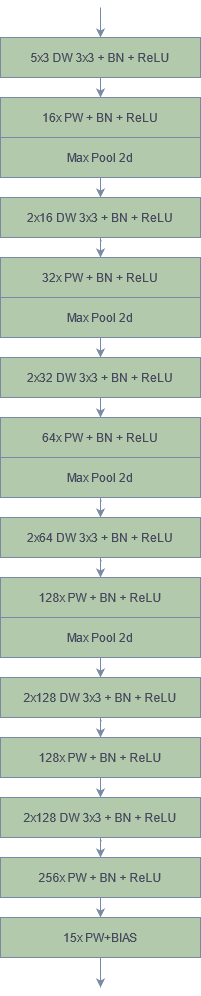
\includegraphics[width=4cm]{images/LNv1}
    \caption{Proponowana architektura sieci \emph{LittleNet}.}
    \label{fig:LN_arch}
\end{figure}

Rozmiar wejścia sieci ustalono na 360 pikseli szerokości oraz 180 pikseli wysokości.
Funkcja błędu odpowiedzi sieci \eqref{eq:loss_yolo_v2} rozszerzono o regularyzację normą $L_1$ parametrów sieci $p$, uzyskując równanie \eqref{eq:loss_yolo_v2_reg}. .
\begin{equation}
\begin{aligned}
loss =& \lambda_{validity} BCE(y_{pred}_{0:2,:,:}, y_{ref}_{0:2,:,:}) \\
&+ \lambda_{bbox} loss_{bbox}(y_{pred}_{3:14,:,:}, x_c,y_c,w,h)\\
&+ \lambda_{reg} L_1(p)
\end{aligned}
\label{eq:loss_yolo_v2_reg}
\end{equation}
Za funkcję błędu regresji $loss_{bbox}$  przyjęto funkcję \emph{GCIoU} daną równaniem \eqref{eq:gciou}. 
Funkcja ta bazuje na \emph{GIoU}\cite{giou}, \emph{DIoU}\cite{dciou} oraz \emph{CIoU}\cite{dciou}. 
Połączenie powyższych funkcji pozwala na połączenie ich zalet funkcji: 
\begin{itemize}
    \item \emph{GIoU} - bardziej bezpośredni wpływ błędu na parametry (gdy \emph{IoU}$ = 0$),
    \item \emph{DIoU} - centralizacji predykcji,
    \item \emph{CIoU} - wzmocnione finalne skalowanie rozmiaru. 
\end{itemize}
\begin{equation}
GCIoU = GIoU + CIoU + IoU - 1
\label{eq:gciou}
\end{equation}
Ustalono parametry wagowe na $\lambda_{validity} = 20$, $\lambda_{bbox} = 1$ oraz $\lambda_{reg} = 0.01$.
Krok uczący został początkowo ustalony jako $l_r=1$. 
W trakcie procesu uczenia podlegał on modyfikacją zgodnie z równaniami \eqref{eq:lr_1} oraz \eqref{eq:lr_2}.
\begin{equation}
l_r_(t+1) = 
\begin{cases}
    1.3*l_r(t), &\text{if } loss(t) < loss(t-1) \\
    0.5*l_r(t), &\text{if } loss(t) > loss(t-1) \\
    l_r(t), &\text{otherwise}
\end{cases}
\label{eq:lr_1}
\end{equation}
\begin{equation}
l_r(t+1) = max(10^{-5}, min(1, l_r(t+1)))
\label{eq:lr_2}
\end{equation}


Po zakończeniu procesu uczenia modelu zmiennoprzecinkowego osiągnięto wartość $iou = 0.8$ dla zbioru walidacyjnego oraz $0.7$ dla zbioru uczącego. 
Powodem tak znacznej różnicy wartości metryki jest znaczny stopień augmentacji danych.

Sieć poddano kwantyzacji. Dane wejściowe zostały poddane kwantyzacji 8 bitowej bez znaku i bez części całkowitej.
Warstwy pośrednie poddano kwantyzacji 8 bitowej ze znakiem i 2 bitami części całkowitej.
Ostatnią warstwę poddano kwantyzacji 8 bitowej ze znakiem i 3 bitami części całkowitej.

Uzyskano wartość $iou = 0.76$ dla zbioru walidacyjnego oraz $0.67$ dla zbioru uczącego.
Na rysunkach \ref{fig:float_loss}-\ref{fig:quant_iou} przedstawiono przebiegi funkcji błędu oraz metryki \emph{IoU} dla modelu zmiennoprzecinkowego oraz kwantyzowanego.

\begin{figure}
     \centering
     \begin{subfigure}[b]{0.49\textwidth}
         \centering
         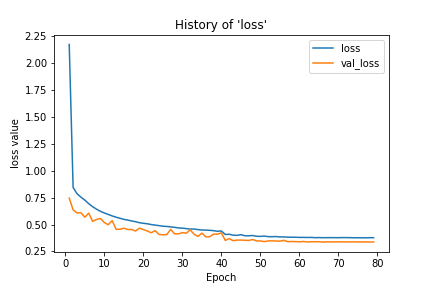
\includegraphics[width=\textwidth]{images/float32_hist_of_loss.png}
         \caption{}
         \label{fig:float_loss}
     \end{subfigure}
     \hfill
     \begin{subfigure}[b]{0.49\textwidth}
         \centering
         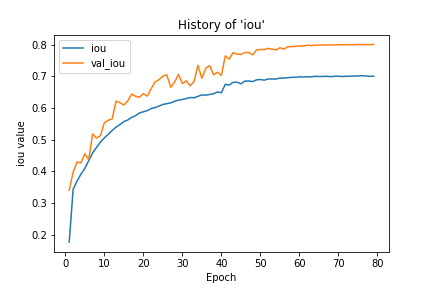
\includegraphics[width=\textwidth]{images/float32_hist_of_iou.png}
         \caption{}
         \label{fig:float_iou}
     \end{subfigure}
     \hfill
     \begin{subfigure}[b]{0.49\textwidth}
         \centering
         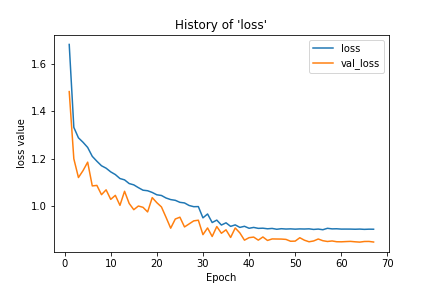
\includegraphics[width=\textwidth]{images/8_bit_quant_hist_of_loss.png}
         \caption{}
         \label{fig:quant_loss}
     \end{subfigure}
     \hfill
     \begin{subfigure}[b]{0.49\textwidth}
         \centering
         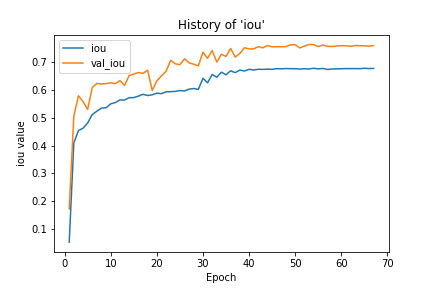
\includegraphics[width=\textwidth]{images/8_bit_quant_hist_of_iou.png}
         \caption{}
         \label{fig:quant_iou}
     \end{subfigure}
     \hfill
     
    \caption{Przebiegi wartości błędu oraz metryki \emph{IoU} (w zależności od epoki uczącej) dla modelu zmiennoprzecinkowego \ref{fig:float_loss} i \ref{fig:float_iou} oraz \ref{fig:quant_loss} i \ref{fig:quant_iou}.}
    \label{fig:two_step_train}
\end{figure}


W trakcie realizacji implementacji sprzętowej, ustalono, iż dla obecnego rozmiaru wejścia sieci nie jest możliwe buforowanie wyników warstw pośrednich w pamięci BRAM.
Z tego względu zdecydowano się na redukcję rozmiaru wejścia sieci do 200 pikseli szerokości oraz 100 pikseli wysokości. 
Rozpoczęto trening sieci z takimi samymi parametrami (wagi sieci zostały wylosowane).  
Uzyskano wartość $iou = 0.78$ dla zbioru walidacyjnego oraz $0.69$ dla zbioru uczącego.
Od epoki $75$ rozpoczęto kwantyzację z wyłączeniem warstw normalizujących.
Względem poprzedniego modelu zmieniono liczbę bitów części całkowitej: 1 dla wyjść oraz 3 dla wag warstw pośrednich.
Następnie od epoki $109$ kwantyzacji poddano również warstwy normalizujące.
Dla modelu w pełni kwantyzowanego uzyskano wartość $iou = 0.71$ dla zbioru walidacyjnego oraz $0.64$ dla zbioru uczącego. Na rysunkach \ref{fig:small_loss}-\ref{fig:small_iou} przedstawiono przebiegi funkcji błędu oraz metryki \emph{IoU} dla modelu o zmniejszonych rozmiarach wejścia. 

\begin{figure}
     \centering
     \begin{subfigure}[b]{0.49\textwidth}
         \centering
         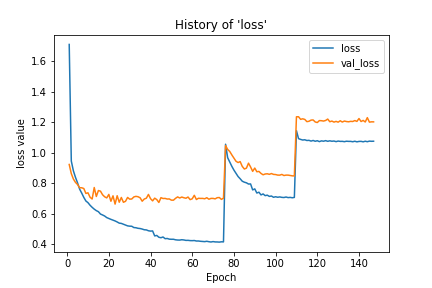
\includegraphics[width=\textwidth]{images/LN_smaller_hist_of_loss.png}
         \caption{}
         \label{fig:small_loss}
     \end{subfigure}
     \hfill
     \begin{subfigure}[b]{0.49\textwidth}
         \centering
         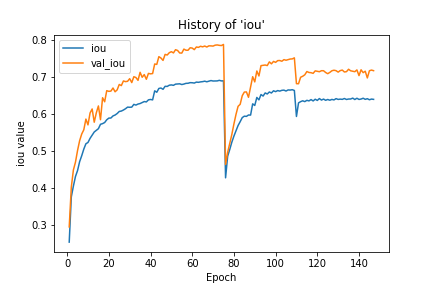
\includegraphics[width=\textwidth]{images/LN_smaller_hist_of_iou.png}
         \caption{}
         \label{fig:small_iou}
     \end{subfigure}
     
    \caption{Przebiegi wartości błędu \ref{fig:small_loss} oraz metryki \emph{IoU} \ref{fig:small_iou} (w zależności od epoki uczącej) dla modelu o rozmiarze wejścia 200x100 pikeli.
    Epoka 75 - rozpoczęcie kwantyzacji bez warstw normalizacyjnych. Epoka 109 - pełna kwantyzacja.}
    \label{fig:three_step_train}
\end{figure}


%  Podsumowanie
Poprzez analizę przeprowadzonych badań architektury stwierdzono, iż stosowanie konwolucji separowalnych posiada zaletę w postaci stosunkowo nie wielkiej liczby parametrów, lecz również wadę wynikającą ze stosunkowo niewielkiego stopnia ekstrakcji cech z danych wejściowych (w szczególności w warstwach początkowych). 
Problem ten rozwiązano poprzez wielokrotną filtrację filtrami typu depthwise.
Ponadto zastosowanie warstw normalizacyjnych pozwoliło na przyspieszenie procesu uczenia.
Wykorzystując wnioski z przeprowadzonych badań zaprojektowano architekturę \emph{LittleNet}. 
Osiągnięto dokładność $iou = 0.71$ wraz ze stosunkowo łatwą implementacją sprzętową.